\section{System Design}

\paragraph{}In this System Customer Request in Text Format To Service Call Center for classify the Request into different categories listed below:\\
1. New vehicle purchase enquiries ( i.e., Enquiry on latest or future or existing product features, price, availability, closest showroom to drop in for purchase or exchange, etc.)\\
2. Test drive requests ( i.e., Request for booking test drives, follow up Request with customers to schedule the same, confirmation that test drive has been done as per schedule or with delayed schedule, etc.)\\
3. Breakdown ( i.e., Customer Send Request TO  contact center to report vehicle break down and providing his location details for repair or breakdown assistance, Road assistance mechanic reaching out to customer and reaching location with preliminary input on vehicle condition )\\
4. Feedback ( Feedback collected post sales /service on vehicle delivery on customer sales/ service experience)\\
5. Vehicle Quality ( Complaints of the vehicle parts not functioning properly, repetitive complaints, etc. - except breakdowns and failures.\\



\subsection{System Architecture}
\paragraph{}The architecture of the proposed system is shown in figure \ref{fig:block_diagram}. It has four modules explained as follows:
\begin{figure}[!h]
\begin{center}
\fbox\{includegraphics[width=1.01\linewidth]{./arch}}
\caption{System Architecure}
\label{fig:block_diagram}
\end{center}
\end{figure}
\newpage
\begin{enumerate}
	

\item New vehicle purchase enquiries ( i.e., Enquiry on latest or future or existing product features, price, availability, closest showroom to drop in for purchase or exchange, etc.)
\item Test drive requests ( i.e., Request for booking test drives, follow up Request with customers to schedule the same, confirmation that test drive has been done as per schedule or with delayed schedule, etc.)
\item Breakdown ( i.e., Customer Send Request TO  contact center to report vehicle break down and providing his location details for repair or breakdown assistance, Road assistance mechanic reaching out to customer and reaching location with preliminary input on vehicle condition )
\item Feedback ( Feedback collected post sales /service on vehicle delivery on customer sales/ service experience)
\item Vehicle Quality ( Complaints of the vehicle parts not functioning properly, repetitive complaints, etc.  except breakdowns and failures
\end{enumerate}

\subsection{Mathematical Model}
\begin{enumerate}
	\item Identify the Users,\\
	U = $\{ u1, u2, u3, ... \}$\\
	Where `U' is main set of Users like u1, u2, u3, ...
	
	\item D be the set of Data.\\
	D = $\{ D1, D2, D3, ... \}$
	
	\item input video\\
	Q = $\{ V1, V2, V3, ... \}$\\
	Where `V' is main set of Video v1, v2, v3, ...
	
	\item SYS = $\{$DX, DF, AP, BG $\}$
	\begin{itemize}
		\item DX = It Data Extractor which extract the data from the dataset.
		\item DF = find fire images using YOLOV3 in database.
		\item AP = Filter the results of YOLOV3 using Algorithm.
		\item BG = It generate the different frame
		
	\end{itemize}
	\item Identify the processes as P.\\
	P = $\{ P1, P2, P3, P4 \}$
	\begin{itemize}
		\item P1 = $\{ e1, e2 \}$ where,\\
		$\{$ e1 = i $|$ i, database designing from the dataset  $\}$\\
		$\{$ e2 = j $|$ j, show all clicks through data from the database  $\}$
		\item P2 = $\{ e1, e2, e3, e4 \}$ where,\\
		$\{$ e1 = i $|$ i, Take the video from the user t $\}$\\
		$\{$ e2 = i $|$ i, Search query using volov3 $\}$\\
		$\{$ e3 = j $|$ j, Filter the results of volov3 using Apriori $\}$\\
		$\{$ e4 = j $|$ j, Generate the frame $\}$\\
		Graph G = $\{ E, V \}$ where,
		\begin{itemize}
			\item[$\ast$] V = $\{ v1, v2, v3, ... \}$ be set of vertex
			\item[$\ast$] E = $\{ (v1,v2), (v2,v3) \}$ be set of edges
		\end{itemize}
		\item P3 = $\{ e1, e2 \}$ where,\\
		$\{$ e1 = i $|$ i, Find out the fire and gun images in video $\}$\\
		
		
		
	\end{itemize}
\end{enumerate}


\subsection{Data Flow Diagram}
\paragraph{}A data flow architecture represents graphical view of flow of data through an information system and modelling its process aspects. This are a preliminary step used to create an overview of the proposed system which can be elaborated later. Data flow architecture (Data Flow Diagram) can also be used for the visualization of data processing of system.\\
%\vspace{.25in}

\paragraph{DFD Level 0: }This is called fundamental level DFD for proposed system. It represents the entire system element as a single bubble with inputs and outputs. Input is the query submitted by user and output is nothing but the suggested queries. Figure \ref{fig:DFD0} is the Level 0 DFD for the system.\\
\begin{figure}[!h]
	\centering
	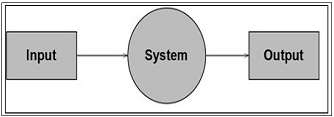
\includegraphics[width=0.725\linewidth]{./dfd0}
		\caption[Level 0 DFD]{Level 0 DFD}
		\label{fig:DFD0}
\end{figure}



\paragraph{DFD Level 1: }This is called as Advanced level DFD for proposed system. It represents systems entire process activities and inputs, outputs in DFD Level 0 will remain same for DFD level 1. The DRec algorithm will accept user query, perform all required operations and returns final suggestions to the user. It consists of user validation, Data extractor, Graph generator, Heat diffusion model and last is the heat value calculation by the random jump. The user is validated, then the user enters a query, using the given query data is extracted from the database, and using a graph generator Query-URL bipartite graph is generated, after applying heat diffusion on it, heat values are calculated by random jump, and those queries having the highest value of heat are suggested to the user. Figure \ref{fig:DFD1} is the Level 1 DFD of the system.
\begin{figure}[!h]
	\centering
	\fbox{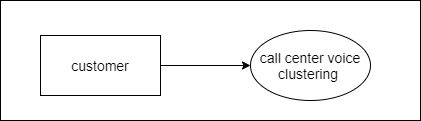
\includegraphics[scale=.725]{./dfd1}}
	\caption{Level 1 DFD}
	\label{fig:DFD1}
\end{figure}
\paragraph{DFD Level 2: }This is called as Advanced level DFD for proposed system. It represents systems entire process activities and inputs, outputs in DFD Level 0 will remain same for DFD level 2. The DRec algorithm will accept user query, perform all required operations and returns final suggestions to the user. It consists of user validation, Data extractor, Graph generator, Heat diffusion model and last is the heat value calculation by the random jump. The user is validated, then the user enters a query, using the given query data is extracted from the database, and using a graph generator Query-URL bipartite graph is generated, after applying heat diffusion on it, heat values are calculated by random jump, and those queries having the highest value of heat are suggested to the user. Figure \ref{fig:DFD2} is the Level 2 DFD of the system.
\begin{figure}[!h]
	\centering
	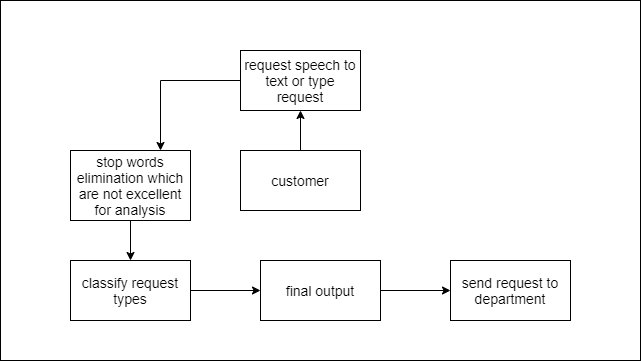
\includegraphics[scale=.725]{./dfd2}
	\caption{Level 2 DFD}
	\label{fig:DFD2}
\end{figure}
\newpage
\subsection{UML Diagrams}
\subsubsection{Use Case Diagram}
\paragraph{}Use case diagram is a list of steps, typically defining interactions between a role (known in UML as an actor) and a system, to achieve a goal. In systems engineering, use cases are used at a higher level than within software engineering, often representing missions or stakeholder goals. The detailed requirements may then be captured in
SysML or as contractual statements. A use case diagram represents all different types of users and all the various ways in which they can interact with the system. Thus, it helps providing a high level view of the system. It is a graphical representation of what the system must accomplish. Use case diagrams help in capturing user requirements, validating design, and generating test cases. Use case diagram for current system is shown in figure \ref{fig:Usecase}.
\vspace{.25in}
\begin{figure}[!h]
\centering
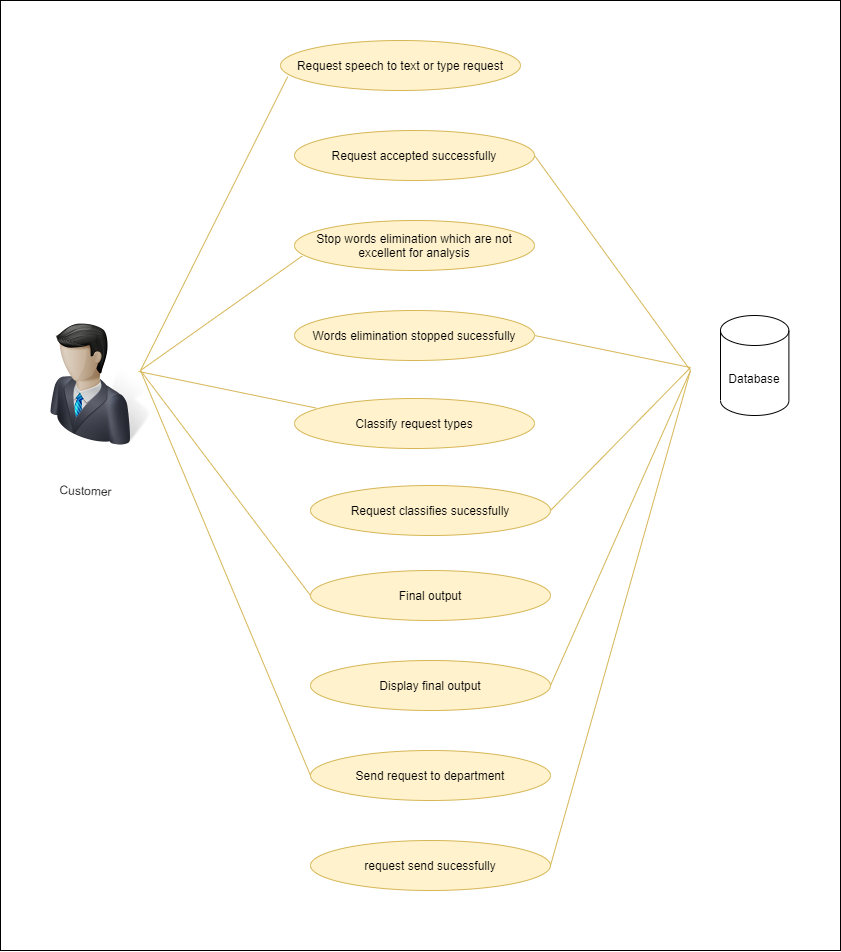
\includegraphics[width=.85\linewidth]{./usecase}
\caption{Use case Diagram}
\label{fig:Usecase}
\end{figure}

\subsubsection{Class Diagram}
\paragraph{}Class diagram describes the structure of a system by showing the system's classes, their attributes, and the relationships among the classes. Proposed system contains seven different types of classes and each posses their own attributes and methods. Main Classes of the proposed system are RandomJump, DBconnection, DFS, Bipartitegraph and HDModel each have different functionalities. Class diagram for proposed system is in figure \ref{fig:Class}.
\begin{figure}[!h]
\centering
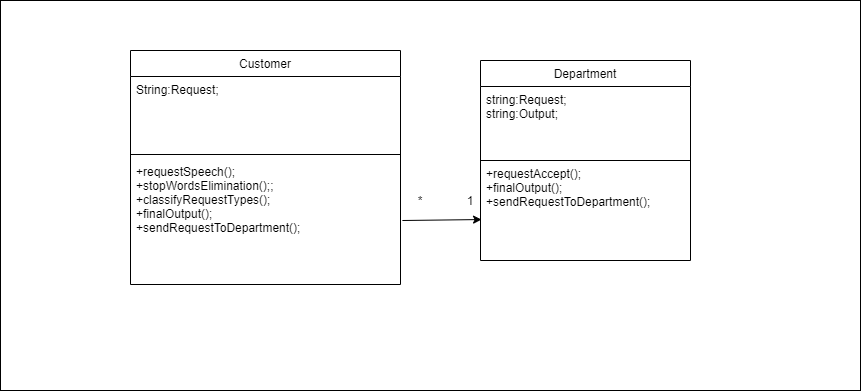
\includegraphics[width=1.0\linewidth]{./Class}
\caption[Class Diagram]{Class Diagram}
\label{fig:Class}
\end{figure}
\newpage
\subsubsection{Activity Diagram}
\paragraph{}An activity is particular operation of the system. An activity diagram is intended to represent stepwise work-flow of activities or actions that can take place in the system. It shows overall flow of control and models computational and organizational processes. Activity diagrams are used to model dynamic aspects of the system. Activity diagram for the system is shown in figure \ref{fig:Activity}.
\begin{figure}[!h]
\centering
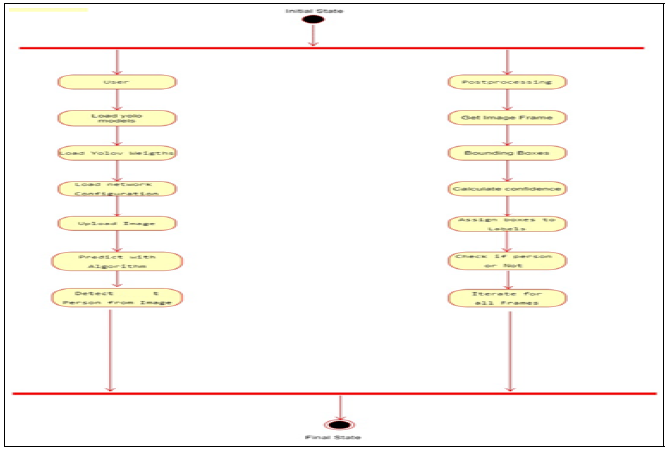
\includegraphics[width=1.1\linewidth]{./act}
\caption{Activity Diagram}
\label{fig:Activity}
\end{figure}
\newpage
\subsubsection{Sequence Diagram} 
\paragraph{}Sequence diagram shows how objects communicate with each other in terms of a sequence of messages. It also indicates the lifespans of objects relative to those messages. There are mainly three different objects User, Recommender system and Database. User enters query, recommender system extracts suggestions from the database using diffusion model and provide results to the user. Figure \ref{fig:Sequence} is sequence diagram for the proposed system.

\begin{figure}[!h]
\centering
\fbox{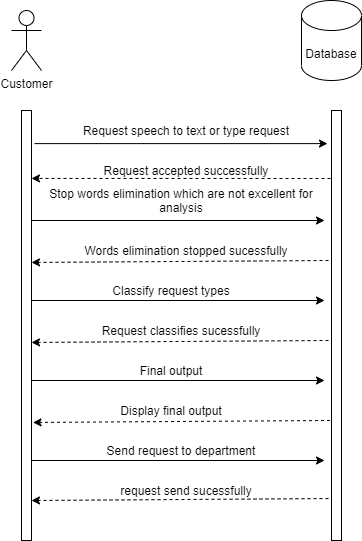
\includegraphics[width=0.88\linewidth]{./Seq}}
\caption{Sequence Diagram}
\label{fig:Sequence}
\end{figure}
\newpage

\subsubsection{State Chart}
\paragraph{}UML state chart describes the states and state transitions of the system. There are many different states through which system transits. First of all user enters a query, system extracts a query-URL bipartite graph from the database, Heat diffusion model is applied over the graph, heat values are calculated after doing random jump and the suggestions to the given query, having top heat values are supplied to user. Figure \ref{fig:Statechart} shows the respective diagram.
%\begin{figure}[!h]
%\centering
%\fbox{\includegraphics[width=0.75\linewidth]{./Statechart}}
%\caption{State Chart}
%\label{fig:Statechart}
%\end{figure}
\newpage
\subsubsection{Component Diagram}
\paragraph{}Component diagram is different than other UML diagrams. Instead of depicting functionality of the system, a component diagram describes how a system is composed by combining different components together. A component diagram describes structural relationship between different components of the system, what are the required interfaces, etc. Components may include executable files, library files, database tables, etc. Component diagram for the system is shown in figure \ref{fig:Component}.
\vspace{.25in}
\begin{figure}[h!]
\centering
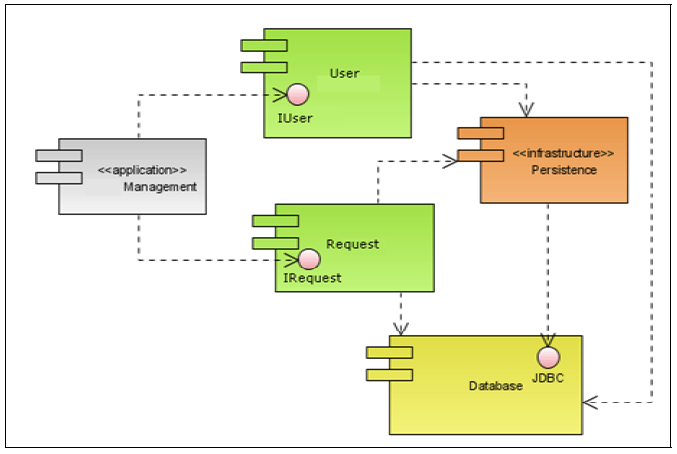
\includegraphics[width=.95\linewidth]{./comp}
\caption{Component Diagram}
\label{fig:Component}
\end{figure}


\newpage
\subsection{Algorithmic Strategy}
\paragraph{} In our project we use TF*IDF algorithm is an information retrieval technique that weighs a term’s frequency (TF) and its inverse document frequency (IDF). Each word or term that occurs in the text has its respective TF and IDF score.\\
The product of the TF and IDF scores of a term is called the TF*IDF weight of that term. Put simply, the higher the TF*IDF score (weight), the rarer the term is in a given document and vice versa.\\
The TF*IDF algorithm is used to weigh a keyword in any content and assign importance to that keyword based on the number of times it appears in the document. More importantly, it checks how relevant the keyword is throughout the web, which is referred to as corpus.\\

Gather words. Write your content. Run a TF*IDF report for your words and get their weights. The higher the numerical weight value, the rarer the term. The smaller the weight, the more common the term. Compare all the terms with high TF*IDF weights with respect to their search volumes on the web. Select those with higher search volumes and lower competition. Work smart.\\

A good rule of thumb is, the more your content “makes sense” to the user, the more weight it is assigned by the search engine. With words having a high TF*IDF weight in your content, your content will always be among the top search results, so you can:\\

stop worrying about using the stop-words.\\
successfully hunt words with higher search volumes and lower competition\\
be sure to have words that make your content unique and relevant to the user, etc.



\subsection{Time Complexity of Proposed System}
\paragraph{}The computation of $e^{\alpha R}$ is very time consuming, so discrete approximation of $e^{\alpha R}$ is used (Equation 3), where P is a positive integer. Two techniques are introduced to reduce the computational complexity (1) since f(0) is a vector, $(I + \frac{\alpha}{p}R)^{p}f(0) $ is calculated iteratively by applying the operator $(I + \frac{\alpha}{p}R)$ to f(0); (2) for matrix R, a data structure is employed which only stores the information of non-zero entries, since it is a very sparse matrix. Thus, supposing a graph is connected by M edges (relationships between nodes), the complexity of executing the heat diffusion process is O(PM), which represents the number of iterations P multiplied by the number of edges M in a graph. In most cases, P = 10 is enough for approximating the heat diffusion equation. The complexity O(PM) shows that the heat diffusion algorithm enjoys very good performance in scalability since it is linear with respect to the number of edges in the graph.